\chapter{Technology Overview} \label{chap:tech} %% chapter 3
\hspace {5mm}

%% ADD LINK TO sections
After a brief introduction, encompassing the history, and some of the requirements in the technologies that support the developed work, this chapter focuses on giving a detailed description of the infrastructure supporting 
the developed work. This chapter is organized in the following matter: in the first section, we focus on SDN/NFV platforms, and the OpenFlow platform; in the second section, an introduction to cloud computing is the main topic,
while also clarifying some of concepts of containerization and virtualization, and how these techniques support the SDN model; in section three, some methods of describing links are explained; in section four, there is an 
analysis of how to monitor and control the SDN platform; and finally in section five we describe how some databases can serve as a backend, and also presenting some interesting new alternatives to the most common ones.

\section {SDN / NFV}

\begin{figure}[!tbph]
  \centering
  {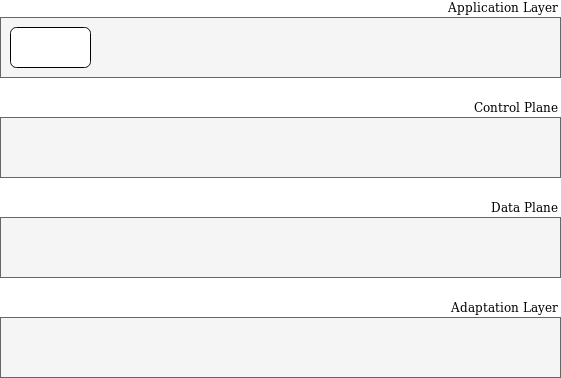
\includegraphics[width=0.6\textwidth]{technology/sdnlayers}\label{fig:net_trad}}
\end{figure}

Given that this chapter focuses on a more technical view of the technologies supporting the various components of the developed system, the previous image is defining the logical separation between layers, the relationship between 
these layers, and the protocols used for connection. In a general case, we can define two essential regions: \textbf{Southbound}, 
providing interfaces between controller and data plane; and \textbf{Northbound}, providing connection between the network infrastructure, and applications and services.

\subsection {Southbound}
\subsubsection {OpenFlow}

One of the most important components of current SDN technologies, and one of the key components that allowed for the proliferation of SDN platforms, OpenFlow is a protocol that was released in order to improve experimentation
in networks, due to a lack of inovation in this field. The way this problem was approached was to develop a protocol that allowed for the creation of programmable networks, also decreasing dependency on closed hardware platforms.

\begin{figure}[!tbph]
  \centering
  {\includegraphics[width=0.6\textwidth]{technology/openflowopenflowlabel{fig:net_trad}}
\end{figure}

\section {Cloud computing}
\section {Link discovery and control}
\section {Infrastructure Management/ Configuration}
\subsection {Data Models}
\subsection {Management Protocols}
\subsubsection {NETCONF}
\subsubsection {gRPC}

%% PRESENT PROMETHEUS
